\documentclass[a4paper]{article}
% \usepackage{thesis}
% define the title
\author{Glen Berseth, Ravjot Singh}
\title{ARM Game: Asynchronous Real-time Multiplayer Game}

\usepackage{epsfig}
\usepackage{amssymb}
\usepackage{amsmath}
\usepackage{amsfonts}
\usepackage{xspace}
\usepackage{named}
\usepackage{hyperref}
\usepackage{booktabs}
\usepackage{float}
\usepackage{wrapfig}
% \usepackage{cite}
%\usepackage{jneurosci}
% \usepackage{natbib}

\usepackage{graphicx}

\usepackage{algorithm2e}
% \usepackage{algorithm}
\usepackage{multirow}
\usepackage{verbatim}
\usepackage{soul}
\usepackage{array}
\setlength\extrarowheight{2pt} % or whatever amount is appropriate

% I am having a hell of a time getting text colouring working in this document
\usepackage[table]{xcolor}
\usepackage{array,hhline}
\usepackage{tikz}
\usetikzlibrary{calc}
\usetikzlibrary{decorations.pathmorphing}
% \usepackage{beamer}
\usepackage{caption}
\usepackage{siunitx}
% \sisetup{output-exponent-marker = E,round-mode = figures, round-precision = 3,
%  scientific-notation = true}
\sisetup{fixdp,dp=3}

% \usepackage[framed,numbered,autolinebreaks,useliterate]{mcode}

% \documentclass{minimal}
\usepackage{soul}
\usepackage{tikz}
\usetikzlibrary{calc}
\usetikzlibrary{decorations.pathmorphing}

\makeatletter

\newcommand{\defhighlighter}[3][]{%
  \tikzset{every highlighter/.style={color=#2, fill opacity=#3, #1}}%
}

\defhighlighter{yellow}{.5}

\newcommand{\highlight@DoHighlight}{
  \fill [ decoration = {random steps, amplitude=1pt, segment length=15pt}
        , outer sep = -15pt, inner sep = 0pt, decorate
        , every highlighter, this highlighter ]
        ($(begin highlight)+(0,8pt)$) rectangle ($(end highlight)+(0,-3pt)$) ;
}

\newcommand{\highlight@BeginHighlight}{
  \coordinate (begin highlight) at (0,0) ;
}

\newcommand{\highlight@EndHighlight}{
  \coordinate (end highlight) at (0,0) ;
}

\newdimen\highlight@previous
\newdimen\highlight@current

\DeclareRobustCommand*\highlight[1][]{%
  \tikzset{this highlighter/.style={#1}}%
  \SOUL@setup
  %
  \def\SOUL@preamble{%
    \begin{tikzpicture}[overlay, remember picture]
      \highlight@BeginHighlight
      \highlight@EndHighlight
    \end{tikzpicture}%
  }%
  %
  \def\SOUL@postamble{%
    \begin{tikzpicture}[overlay, remember picture]
      \highlight@EndHighlight
      \highlight@DoHighlight
    \end{tikzpicture}%
  }%
  %
  \def\SOUL@everyhyphen{%
    \discretionary{%
      \SOUL@setkern\SOUL@hyphkern
      \SOUL@sethyphenchar
      \tikz[overlay, remember picture] \highlight@EndHighlight ;%
    }{%
    }{%
      \SOUL@setkern\SOUL@charkern
    }%
  }%
  %
  \def\SOUL@everyexhyphen##1{%
    \SOUL@setkern\SOUL@hyphkern
    \hbox{##1}%
    \discretionary{%
      \tikz[overlay, remember picture] \highlight@EndHighlight ;%
    }{%
    }{%
      \SOUL@setkern\SOUL@charkern
    }%
  }%
  %
  \def\SOUL@everysyllable{%
    \begin{tikzpicture}[overlay, remember picture]
      \path let \p0 = (begin highlight), \p1 = (0,0) in \pgfextra
        \global\highlight@previous=\y0
        \global\highlight@current =\y1
      \endpgfextra (0,0) ;
      \ifdim\highlight@current < \highlight@previous
        \highlight@DoHighlight
        \highlight@BeginHighlight
      \fi
    \end{tikzpicture}%
    \the\SOUL@syllable
    \tikz[overlay, remember picture] \highlight@EndHighlight ;%
  }%
  \SOUL@
}
\makeatother

\begin{document}
  Lorem ipsum \highlight{dolor sit amet, consectetur adipis-icing elit, sed do
eiusmod tempor} incididunt ut labore et dolore magna aliqua. Ut enim ad minim
veniam, quis nostrud exercitation \highlight[red]{ullamco $laboris$ nisi ut
aliquip ex ea commodo consequat. Duis aute irure dolor in reprehenderit} in
voluptate velit esse cillum dolore eu fugiat nulla pariatur.  Excepteur sint
occaecat \highlight[green, draw=blue]{cupidatat non proident,
suntinculpaquiofficiadeseruntmollitanimidestlaborum.
Loremipsumdolorsitametconsecteturadipisicingelitseddoeiusmodtemporincididuntutlabore-etdoloremagnaaliqua.}
I suppose I could write some more text here.
\end{document}
% new commands

% common formatting commands
\newcommand{\todo}[1]{\textcolor{red}{Todo:#1}}
\newcommand{\glen}[1]{\textcolor{blue}{Glen:#1}}
\newcommand{\ravjot}[1]{\textcolor{green}{Ravjot:#1}}
\newcommand{\todocite}[1]{\textcolor{red}{[??#1??]}}

\newcommand{\ptoP}{\emph{peer-to-peer}\xspace}
\newcommand{\clientServer}{\emph{client-server}\xspace}


% % % % % % % % Game stuff % % % % % % % % %

% \newcommand{\move}[1]{\ensuremath{move(#1)}\xspace}
\newcommand{\move}[2]{\ensuremath{updateLocation(#1,#2)}\xspace}
\newcommand{\fire}[2]{\ensuremath{fire(#1,#2)}\xspace}
\newcommand{\destroy}[1]{\ensuremath{destroy(#1)}\xspace}
\newcommand{\agent}{\ensuremath{a}\xspace}
\newcommand{\position}{\ensuremath{p}\xspace}
\newcommand{\direction}{\ensuremath{d}\xspace}

% % % % % % % % short forms % % % % % % % % % %
\newcommand{\gamestate}{\emph{gamestate}\xspace}
\newcommand{\gamestates}{\emph{gamestate}s\xspace}
\newcommand{\kvService}{\emph{kvservice}\xspace}
\newcommand{\activityServer}{\emph{activityserver}\xspace}
\newcommand{\localServer}{\emph{localServer}\xspace}
\newcommand{\localServers}{\emph{localServers}\xspace}
\newcommand{\agentstate}{\emph{agentstate}\xspace}
\newcommand{\gameStateConstruction}{\emph{gameStateConstruction}\xspace}
%\enumi
\begin{document}

% generates the title
\maketitle
% insert the table of contents
% \tableofcontents


\begin{abstract}
	 Real-time multiplayer games are complex systems that often have a single point of failure and are not scalable.
	 In this work a prototype design is created to handle node failure during game simulation.
	 The client server paradigm is modified to construct a distributed server at each node.
	 Propagation of \gamestate is performed across nodes keeping each node up to date.
	 Node failure is handled gracefully without noticeable suspension of gameplay.
	 Using distributed state across nodes also shows promise in the area of scalability. 
\end{abstract}


\section{Introduction}
\label{sec:Intro}


We propose to construct a distributed \clientServer in order to support fail-stop scenarios. We assume no limits on bandwidth and have strong constraints on latency. We will use this system to support a simple computer game of a number of agents moving around in a 2D world.

	




\section{Related Work}

Some related work stuff.


\section{Methodology}
\label{sec:methodology}

	In this section we outline our solution to our distributed state synchronization design. We discus what protocols are used, how the clients and servers communicate and the example game constructed for this system.
	
\subsection{The Clients}

	The client locally simulates its own version of the game. To support this the client needs to keep a list of the agents controlled by other clients in the game and the most recent location of each agent. This information will be stored in a \emph{hashmap}. After every frame is rendered in the game the client will broadcast a position update to all servers.
	
\subsection{The Servers}

	The server simulates its own version of the game. The server is not used just to reduce message passing but also to act as an authority over clients, to prevent malicious clients from propagating invalid information.
	
	In the simulation loop for the server a number of actions occur
	\begin{enumerate}[topsep=2pt,itemsep=-1ex,partopsep=1ex,parsep=1ex]
		\item the server accepts event messages and puts them in a queue for processing
		\item The server accepts position updates from clients
		\item The server verifies these updates to be valid
		\item The server's local copy of agent locations is updated
		\item The server processes any events in its event queue
		\item If events are valid, update server's game state and broadcast the result
	\end{enumerate}
	
	This way the server keeps the true state of the game and informs the clients of valid updates to the server's state. To perform these operations the server needs to have state for the currently active clients and its own version of the game state.

\subsection{The Activity Server}
	The purpose of \activityServer is to support the architecture of the system which includes allowing a new node to join the system and publishing the list of nodes which are currently online. The \activityServer doesn't do any kind of game simulation niether get involves in game semantic actions.

\subsection{The Key-Value Service}
	The \kvService is a key-value service which used for all communication among the nodes and the \activityServer that is required to maintain the system. The nodes periodically update their entry in the \kvService. The \activityServer polls with twice the period the rest of the nodes are polling. The \activityServer read the entries of all the nodes and publish a list of nodes including all those nodes who have recently updated their entry. 

\subsection{ARM Game}

	We will simulate a very basic game to use as our state to synchronize. 
	The game has two possible actions \move{\agent}{\position} and \fire{\agent_{i}}{\agent_{j}}. These actions can be executed at any point in the game but the server must validate the actions. 
	
	In order to simulate the game, information is needed on the other agents in the game. The only data stored for each agent is the agent's current location. The information needed for the game will be provided from the server or client the game is being simulated on. Computer animations and therefore game simulations use simulation time, similar to a vector clock, for synchronizing events.
	
\subsubsection{Protocol and Messaging}

	The clients send updates/events to every server. For \fire{\agent_{i}}{\agent_{j}} events the server that is paired with the client with $\agent_{j}$ will determine the outcome. If the \fire{\agent_{i}}{\agent_{j}} event is successful according to the authoritative server a \destroy{\agent_{j}} event is broadcast to every server. All communication is asynchronous without acknowledgements.


\subsection{Distributed Servers}
\label{subsec:distributed-servers}

	We construct a distributed server model (see Figure~\ref{figure:server-models}(b)) to enable better failure handling in our system. Each client is paired with a server which is running on the same machine. The paired server validates the actions performed by client and process it further if the action is found valid. The authoritative server for a particular client depends on the event/action being processed. 
	
	\begin{figure}[ht]
	\centering
	\begin{tabular}{c c}
		Client-Server & Distributed Server \\
		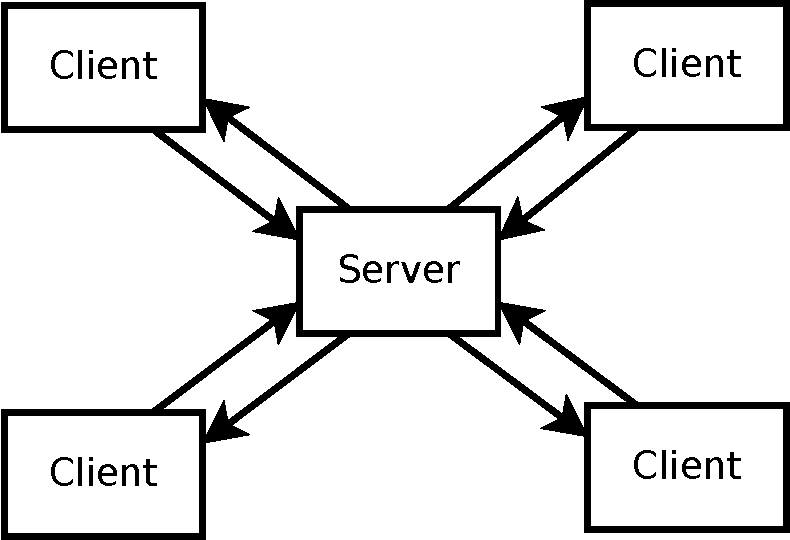
\includegraphics[width=0.44\linewidth]{../images/client-server-model-crop.pdf} &
		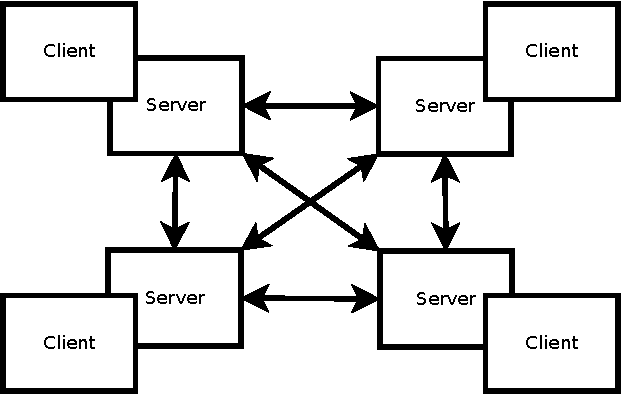
\includegraphics[width=0.48\linewidth]{../images/client-distributed-server-model-crop.pdf} \\
		(a) & (b)
	\end{tabular}

	\caption{\label{figure:server-models} The first model (a) is an example \clientServer model. In this model all of the clients send updates to the server and the server send updates out to the clients. In the second model (b) the server is distributed and clients communicate with many servers.}
	\end{figure}
	




\section{Evaluation}
\label{sec:evaluation}

We plan to evaluate our method in two ways. Primarily, the methods ability to handle failure. To cope with the failure gracefully and cause the least amount of disturbance in the gameplay as possible. A secondary goal is to keep the latency of the game down as more clients and server are added to the system.

\subsection{Fault Tolerance}

The goal of the system was to gracefully cope with failing nodes without introducing latency. 
A game system design may choose to pause the processing of the game until the \gamestate becomes consistent again, during this time the players must wait for the game state to synchronize.
Game flow and minimal latency (as seen from a player of the game) is prioritized for consistency in this project.
In order to reduce latency consistency is sacrificed. 
When a node fails it could take a short amount of time to detect this failure as an inactivity.
During this time the agent for that node still exists in the game but is immobile.

Overall the system works as desired for graceful fault tolerance.
When a node fails the agent exists in the \gamestate for every node for a short period (a few seconds) after which all data related to the agent is removed from the \gamestate.

\subsection{Scalability vs Consistency}

It is difficult to measure the consistency between each of the nodes. 
We would have to employ a large logging system that would take snap shots of the \gamestate at points in time. 
In order for these snapshots to be effective there would need to be additional time synchronization across the nodes for comparison. 
Instead the relative number of successful shots is used to measure consistency. 
A successful shot is one that is initiated by a client, forwarded to the client's local server and again forwarded to the proper server for validation. 
The shot is successful if the last server agrees with the result of the shot. 
The occurrence of successful shot implies that $3$ \gamestates where at least partial consistent.
We measure the scalability by increasing the number of nodes in the system and comparing the relative number of fire events that are successful. 
	\begin{figure}[ht]
	\centering
		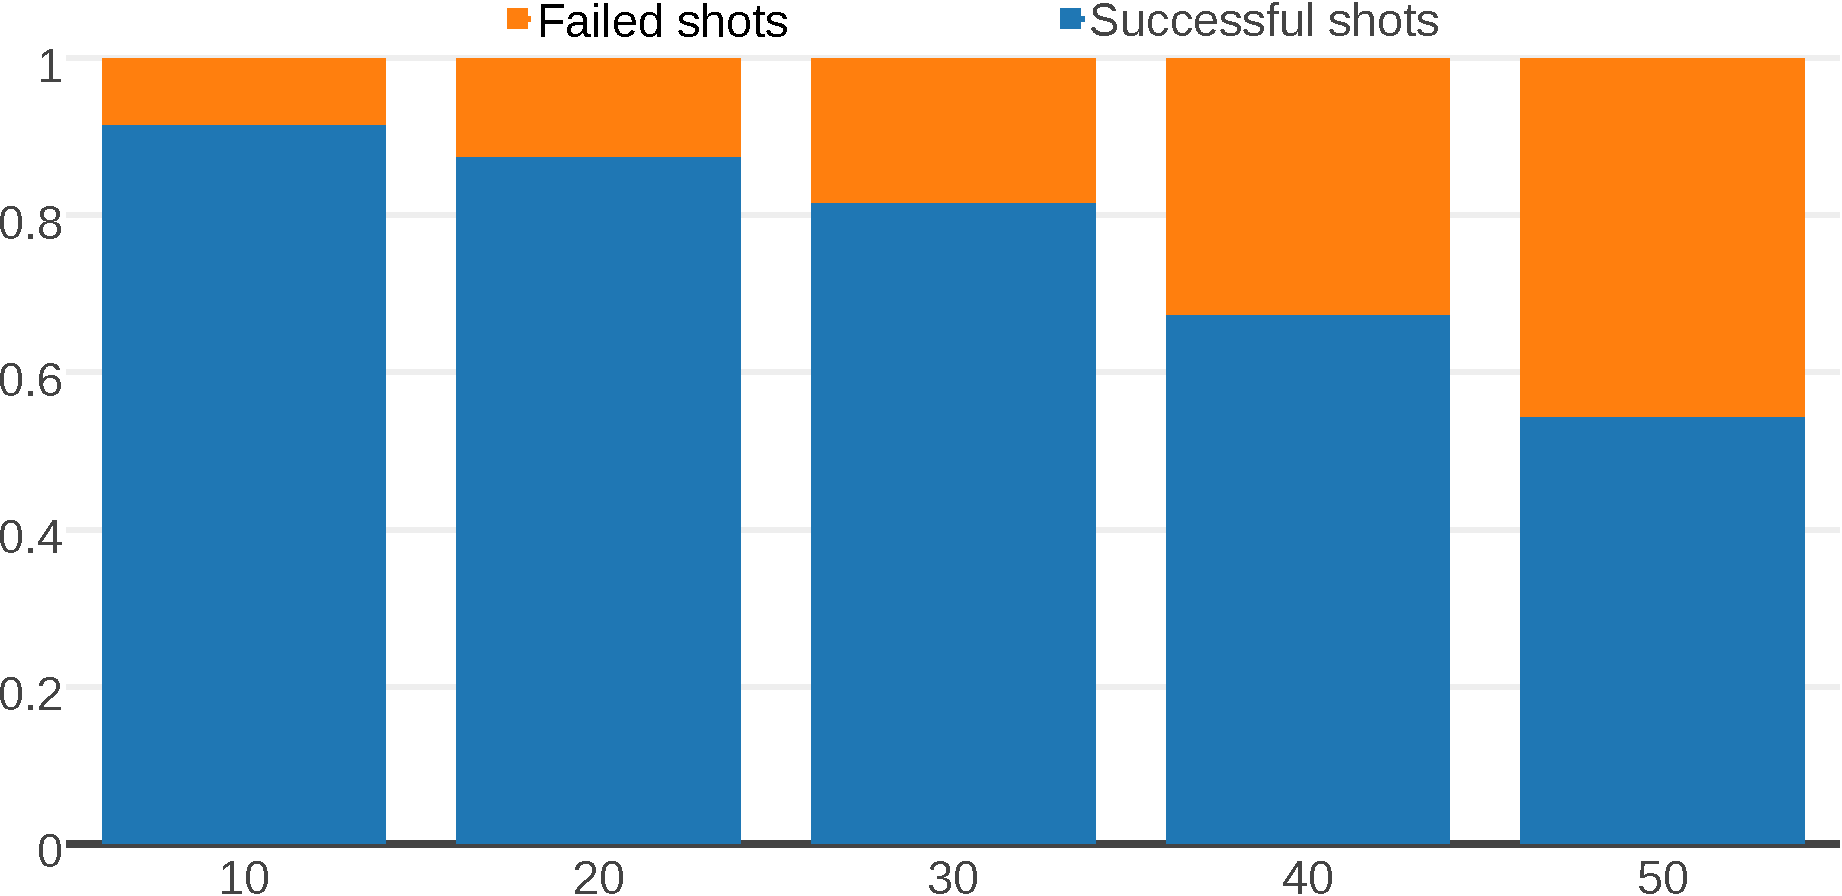
\includegraphics[width=0.95\linewidth]{../images/agents-vs-consistency-via-shots-crop.pdf}
		agents
		\caption{\label{figure:nodes-vs-shots-consistency} A chart of the relative numbers of successful shots vs failed shots. As the number of nodes in the system increases the relative number of successful shots decreases.}
	\end{figure}
Figure~\ref{figure:nodes-vs-shots-consistency} shows us how well the systems consistency copes with the number of nodes in the system. As expected, as the number of nodes increases the number of successful shots decreases. The decrease in successful shots is a proxy for the system consistency. 
This is the result of increased latency and dropped packets in the system. 

\subsection{Game Simulation}

Here a description of the game is given, along with some features of the client Artificial Intelligence. The game is confined to a 3D box of dimensions $10x10x10$. Inside the box all the agents are simulated using a pseudo randomized AI. A visualization of the \gamestate is shown in Figure~\ref{figure:game-renders}(a and b).

\begin{figure}[htb]
\centering
	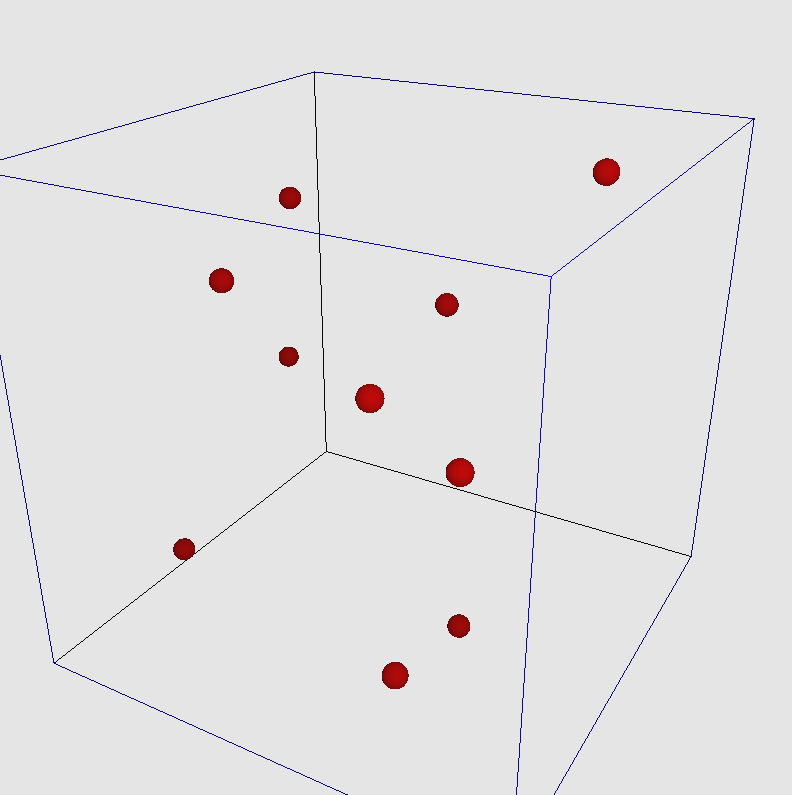
\includegraphics[width=0.45\linewidth]{../images/10-agents-render.png}
	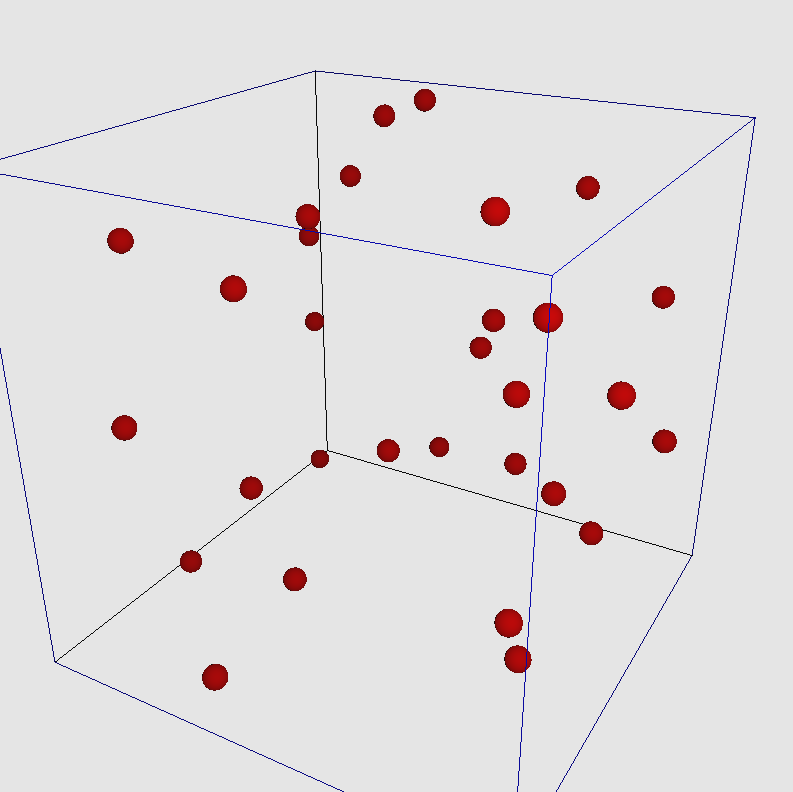
\includegraphics[width=0.45\linewidth]{../images/30-agents-render.png}	

	\caption{\label{figure:game-renders} Two rasterized simulation frames. On the left with $10$ agents and on the right with $30$ agents.}
\end{figure}

\noindent \textbf{RandomAI}: When an agent is initialized the agent is given a random starting position in the game. The agent is also given a random direction that the agent will travel. From this the agent will navigate along that direction of travel and bounce off the walls of the game box.

Each client will send an update of its location every $100ms$ and will update its own internal state every $100ms$ as well. The client can updated its state at faster intervals if desired. Each node will update its status in the \kvService every 2 seconds. The \activityServer will collect the node updates and post the updated list of active nodes every second. If a node dose not post an update for a duration of $6$ seconds, it is removed from the list of active nodes. In Table~\ref{table:gamestate-discription} the data a node stores to support the system is described. The \gamestate takes up the most amount of memory and it the most frequently updated structure.

\begin{table}[htb]
\centering
	\begin{tabular}{p{0.2\linewidth} | p{0.2\linewidth} | p{0.6\linewidth}}
	\textbf{Attribute name} & \textbf{Type} & \textbf{Description} \\ \hline
	\gamestate & map$<$string, Agent$>$ & map of agent identifiers to agent objects in the game \\ \hline
	Nodes & map$<$string, *net.UDPConn$>$ & map of nodes to the UDP connections to send messages to the nodes \\ \hline
	MyClientName & string  & identifier of the client this node is paired with\\  \hline
	ClientLink & *net.UDPAddr & UDP address of the client for this node\\ \hline
	Connection & *net.UDPConn & This nodes UDP listening connection \\ \hline	
	\end{tabular}
	\caption{\label{table:gamestate-discription} Layout of the data stored by each node.}
\end{table}



\section{Timeline}
\label{sec:timeline}

Delivery Dates:
\begin{enumerate}[topsep=2pt,itemsep=-1ex,partopsep=1ex,parsep=1ex]
	\item 21 March: Iteration 1 (Single Server Prototype)
	\item 29 March: Iteration 2 (Distributed Server Prototype)
	\item 05 April: Project Report and Presentation Slides
	\item 12 April: Testing and Refining
\end{enumerate}

\bibliographystyle{named}
\bibliography{project}


%\addcontentsline{toc}{chapter}{Appendix}
% \input{report_appendix}

\end{document}